\documentclass{standalone}
\usepackage{tikz}
\usetikzlibrary{patterns, positioning}

\begin{document}
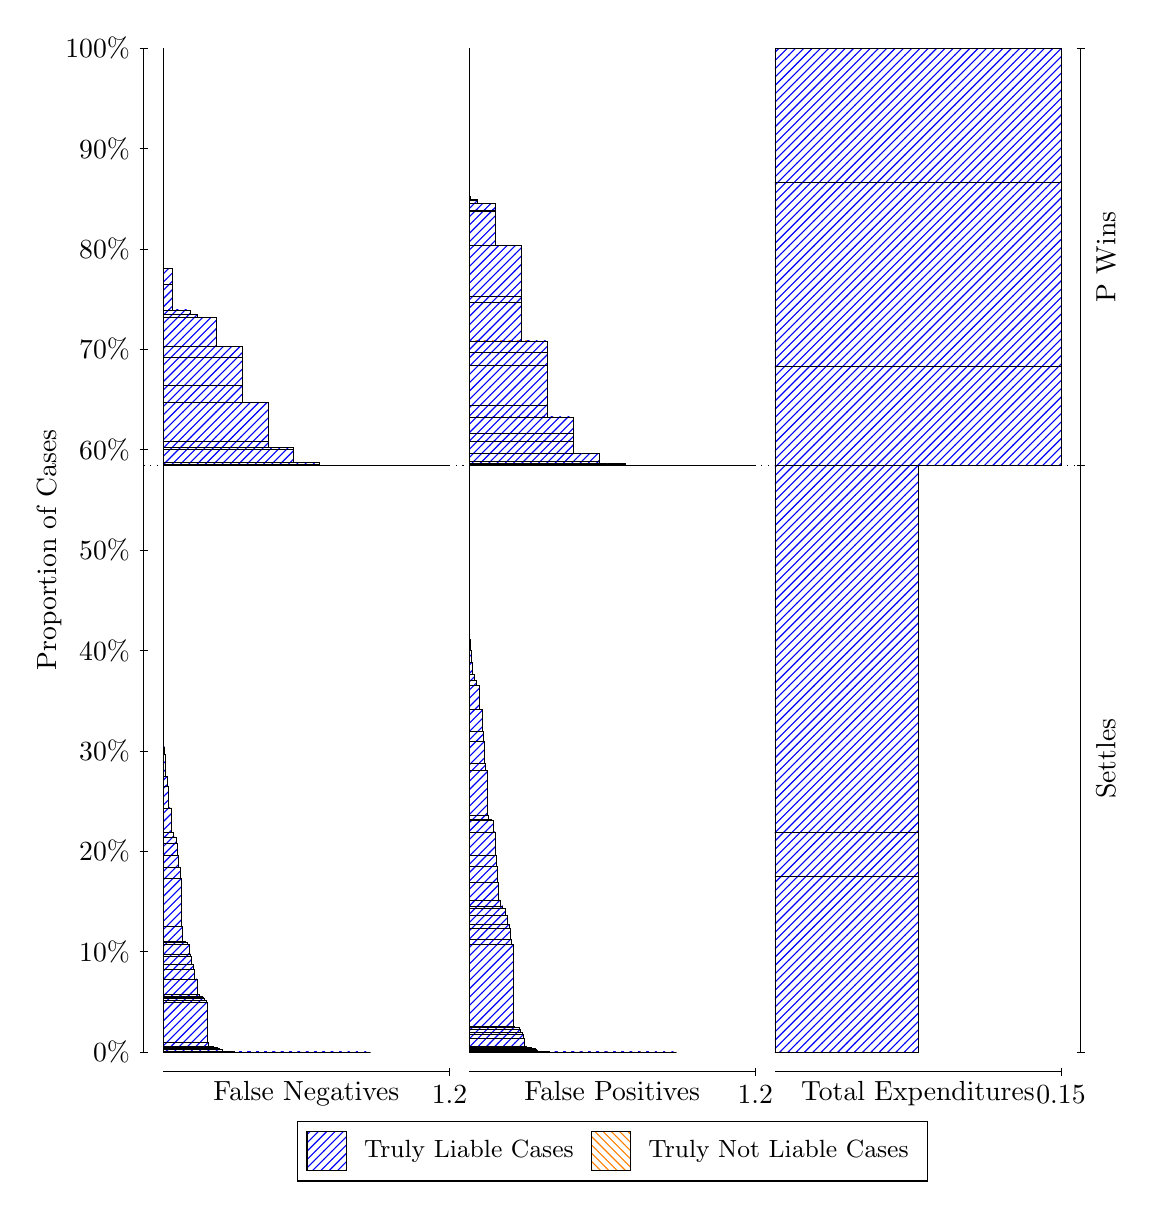
\begin{tikzpicture}
\draw[black, very thin] (1.5,1.75) -- (1.5,14.5);
\node[rotate=90, anchor=center] at (0.3, 8.125) {Proportion of Cases};
\draw[black, very thin] (1.45,1.75) -- (1.55,1.75);
\node[anchor=east] at (1.45, 1.75) {0\%};
\draw[black, very thin] (1.45,3.025) -- (1.55,3.025);
\node[anchor=east] at (1.45, 3.025) {10\%};
\draw[black, very thin] (1.45,4.3) -- (1.55,4.3);
\node[anchor=east] at (1.45, 4.3) {20\%};
\draw[black, very thin] (1.45,5.575) -- (1.55,5.575);
\node[anchor=east] at (1.45, 5.575) {30\%};
\draw[black, very thin] (1.45,6.85) -- (1.55,6.85);
\node[anchor=east] at (1.45, 6.85) {40\%};
\draw[black, very thin] (1.45,8.125) -- (1.55,8.125);
\node[anchor=east] at (1.45, 8.125) {50\%};
\draw[black, very thin] (1.45,9.4) -- (1.55,9.4);
\node[anchor=east] at (1.45, 9.4) {60\%};
\draw[black, very thin] (1.45,10.675) -- (1.55,10.675);
\node[anchor=east] at (1.45, 10.675) {70\%};
\draw[black, very thin] (1.45,11.95) -- (1.55,11.95);
\node[anchor=east] at (1.45, 11.95) {80\%};
\draw[black, very thin] (1.45,13.225) -- (1.55,13.225);
\node[anchor=east] at (1.45, 13.225) {90\%};
\draw[black, very thin] (1.45,14.5) -- (1.55,14.5);
\node[anchor=east] at (1.45, 14.5) {100\%};

\draw[black, very thin] (13.4,1.75) -- (13.4,14.5);
\draw[black, very thin] (13.35,1.75) -- (13.45,1.75);
\node[anchor=west] at (13.35, 1.75) {};
\draw[black, very thin] (13.35,9.1963) -- (13.45,9.1963);
\node[anchor=west] at (13.35, 9.1963) {};
\draw[black, very thin] (13.35,14.5) -- (13.45,14.5);
\node[anchor=west] at (13.35, 14.5) {};

\draw[black, very thin, pattern color=blue, pattern=north east lines] (1.75,1.75) rectangle (4.3823,1.75);
\draw[black, very thin, pattern color=blue, pattern=north east lines] (1.75,1.75) rectangle (4.234,1.75);
\draw[black, very thin, pattern color=blue, pattern=north east lines] (1.75,1.75) rectangle (4.0857,1.75);
\draw[black, very thin, pattern color=blue, pattern=north east lines] (1.75,1.75) rectangle (4.0528,1.75);
\draw[black, very thin, pattern color=blue, pattern=north east lines] (1.75,1.75) rectangle (3.9374,1.75);
\draw[black, very thin, pattern color=blue, pattern=north east lines] (1.75,1.75) rectangle (3.9045,1.75);
\draw[black, very thin, pattern color=blue, pattern=north east lines] (1.75,1.75) rectangle (3.7891,1.75);
\draw[black, very thin, pattern color=blue, pattern=north east lines] (1.75,1.75) rectangle (3.7562,1.75);
\draw[black, very thin, pattern color=blue, pattern=north east lines] (1.75,1.75) rectangle (3.7232,1.75);
\draw[black, very thin, pattern color=blue, pattern=north east lines] (1.75,1.75) rectangle (3.6408,1.75);
\draw[black, very thin, pattern color=blue, pattern=north east lines] (1.75,1.75) rectangle (3.6079,1.75);
\draw[black, very thin, pattern color=blue, pattern=north east lines] (1.75,1.75) rectangle (3.5749,1.75);
\draw[black, very thin, pattern color=blue, pattern=north east lines] (1.75,1.75) rectangle (3.4925,1.75);
\draw[black, very thin, pattern color=blue, pattern=north east lines] (1.75,1.75) rectangle (3.4596,1.75);
\draw[black, very thin, pattern color=blue, pattern=north east lines] (1.75,1.75) rectangle (3.4266,1.75);
\draw[black, very thin, pattern color=blue, pattern=north east lines] (1.75,1.75) rectangle (3.3937,1.75);
\draw[black, very thin, pattern color=blue, pattern=north east lines] (1.75,1.75) rectangle (3.3442,1.75);
\draw[black, very thin, pattern color=blue, pattern=north east lines] (1.75,1.75) rectangle (3.3113,1.75);
\draw[black, very thin, pattern color=blue, pattern=north east lines] (1.75,1.75) rectangle (3.2783,1.75);
\draw[black, very thin, pattern color=blue, pattern=north east lines] (1.75,1.75) rectangle (3.2454,1.75);
\draw[black, very thin, pattern color=blue, pattern=north east lines] (1.75,1.75) rectangle (3.1959,1.75);
\draw[black, very thin, pattern color=blue, pattern=north east lines] (1.75,1.75) rectangle (3.163,1.75);
\draw[black, very thin, pattern color=blue, pattern=north east lines] (1.75,1.75) rectangle (3.13,1.75);
\draw[black, very thin, pattern color=blue, pattern=north east lines] (1.75,1.75) rectangle (3.0971,1.75);
\draw[black, very thin, pattern color=blue, pattern=north east lines] (1.75,1.75) rectangle (3.0641,1.75);
\draw[black, very thin, pattern color=blue, pattern=north east lines] (1.75,1.75) rectangle (3.0476,1.75);
\draw[black, very thin, pattern color=blue, pattern=north east lines] (1.75,1.75) rectangle (3.0147,1.75);
\draw[black, very thin, pattern color=blue, pattern=north east lines] (1.75,1.75) rectangle (2.9817,1.75);
\draw[black, very thin, pattern color=blue, pattern=north east lines] (1.75,1.75) rectangle (2.9488,1.75);
\draw[black, very thin, pattern color=blue, pattern=north east lines] (1.75,1.75) rectangle (2.9158,1.75);
\draw[black, very thin, pattern color=blue, pattern=north east lines] (1.75,1.75) rectangle (2.8993,1.75);
\draw[black, very thin, pattern color=blue, pattern=north east lines] (1.75,1.75) rectangle (2.8664,1.7501);
\draw[black, very thin, pattern color=blue, pattern=north east lines] (1.75,1.7501) rectangle (2.8334,1.7506);
\draw[black, very thin, pattern color=blue, pattern=north east lines] (1.75,1.7506) rectangle (2.8005,1.7507);
\draw[black, very thin, pattern color=blue, pattern=north east lines] (1.75,1.7507) rectangle (2.7675,1.7508);
\draw[black, very thin, pattern color=blue, pattern=north east lines] (1.75,1.7508) rectangle (2.751,1.7508);
\draw[black, very thin, pattern color=blue, pattern=north east lines] (1.75,1.7508) rectangle (2.7345,1.7508);
\draw[black, very thin, pattern color=blue, pattern=north east lines] (1.75,1.7508) rectangle (2.7181,1.7509);
\draw[black, very thin, pattern color=blue, pattern=north east lines] (1.75,1.7509) rectangle (2.6851,1.751);
\draw[black, very thin, pattern color=blue, pattern=north east lines] (1.75,1.751) rectangle (2.6522,1.7533);
\draw[black, very thin, pattern color=blue, pattern=north east lines] (1.75,1.7533) rectangle (2.6192,1.7539);
\draw[black, very thin, pattern color=blue, pattern=north east lines] (1.75,1.7539) rectangle (2.6027,1.7551);
\draw[black, very thin, pattern color=blue, pattern=north east lines] (1.75,1.7551) rectangle (2.5862,1.7556);
\draw[black, very thin, pattern color=blue, pattern=north east lines] (1.75,1.7556) rectangle (2.5698,1.7561);
\draw[black, very thin, pattern color=blue, pattern=north east lines] (1.75,1.7561) rectangle (2.5368,1.7575);
\draw[black, very thin, pattern color=blue, pattern=north east lines] (1.75,1.7575) rectangle (2.5039,1.7809);
\draw[black, very thin, pattern color=blue, pattern=north east lines] (1.75,1.7809) rectangle (2.4709,1.7904);
\draw[black, very thin, pattern color=blue, pattern=north east lines] (1.75,1.7904) rectangle (2.4544,1.8005);
\draw[black, very thin, pattern color=blue, pattern=north east lines] (1.75,1.8005) rectangle (2.4379,1.8071);
\draw[black, very thin, pattern color=blue, pattern=north east lines] (1.75,1.8071) rectangle (2.4215,1.8089);
\draw[black, very thin, pattern color=blue, pattern=north east lines] (1.75,1.8089) rectangle (2.405,1.8145);
\draw[black, very thin, pattern color=blue, pattern=north east lines] (1.75,1.8145) rectangle (2.3885,1.8178);
\draw[black, very thin, pattern color=blue, pattern=north east lines] (1.75,1.8178) rectangle (2.3556,1.8198);
\draw[black, very thin, pattern color=blue, pattern=north east lines] (1.75,1.8198) rectangle (2.3226,1.8681);
\draw[black, very thin, pattern color=blue, pattern=north east lines] (1.75,1.8681) rectangle (2.3061,2.3791);
\draw[black, very thin, pattern color=blue, pattern=north east lines] (1.75,2.3791) rectangle (2.2896,2.4027);
\draw[black, very thin, pattern color=blue, pattern=north east lines] (1.75,2.4027) rectangle (2.2732,2.4279);
\draw[black, very thin, pattern color=blue, pattern=north east lines] (1.75,2.4279) rectangle (2.2567,2.4485);
\draw[black, very thin, pattern color=blue, pattern=north east lines] (1.75,2.4485) rectangle (2.2402,2.4626);
\draw[black, very thin, pattern color=blue, pattern=north east lines] (1.75,2.4626) rectangle (2.2073,2.4845);
\draw[black, very thin, pattern color=blue, pattern=north east lines] (1.75,2.4845) rectangle (2.1743,2.6782);
\draw[black, very thin, pattern color=blue, pattern=north east lines] (1.75,2.6782) rectangle (2.1413,2.801);
\draw[black, very thin, pattern color=blue, pattern=north east lines] (1.75,2.801) rectangle (2.1249,2.8605);
\draw[black, very thin, pattern color=blue, pattern=north east lines] (1.75,2.8605) rectangle (2.1084,2.9675);
\draw[black, very thin, pattern color=blue, pattern=north east lines] (1.75,2.9675) rectangle (2.0919,2.9966);
\draw[black, very thin, pattern color=blue, pattern=north east lines] (1.75,2.9966) rectangle (2.0754,3.1146);
\draw[black, very thin, pattern color=blue, pattern=north east lines] (1.75,3.1146) rectangle (2.059,3.1413);
\draw[black, very thin, pattern color=blue, pattern=north east lines] (1.75,3.1413) rectangle (2.026,3.1545);
\draw[black, very thin, pattern color=blue, pattern=north east lines] (1.75,3.1545) rectangle (1.993,3.3473);
\draw[black, very thin, pattern color=blue, pattern=north east lines] (1.75,3.3473) rectangle (1.9766,3.955);
\draw[black, very thin, pattern color=blue, pattern=north east lines] (1.75,3.955) rectangle (1.9601,4.0987);
\draw[black, very thin, pattern color=blue, pattern=north east lines] (1.75,4.0987) rectangle (1.9436,4.2534);
\draw[black, very thin, pattern color=blue, pattern=north east lines] (1.75,4.2534) rectangle (1.9271,4.4029);
\draw[black, very thin, pattern color=blue, pattern=north east lines] (1.75,4.4029) rectangle (1.9107,4.4819);
\draw[black, very thin, pattern color=blue, pattern=north east lines] (1.75,4.4819) rectangle (1.8777,4.5409);
\draw[black, very thin, pattern color=blue, pattern=north east lines] (1.75,4.5409) rectangle (1.8447,4.8491);
\draw[black, very thin, pattern color=blue, pattern=north east lines] (1.75,4.8491) rectangle (1.8118,5.1294);
\draw[black, very thin, pattern color=blue, pattern=north east lines] (1.75,5.1294) rectangle (1.7953,5.2461);
\draw[black, very thin, pattern color=blue, pattern=north east lines] (1.75,5.2461) rectangle (1.7788,5.5297);
\draw[black, very thin, pattern color=blue, pattern=north east lines] (1.75,5.5297) rectangle (1.7624,5.6248);
\draw[black, very thin, pattern color=orange, pattern=north west lines] (1.75,5.6248) rectangle (1.75,5.6248);
\draw[black, very thin, pattern color=blue, pattern=north east lines] (1.75,5.6248) rectangle (1.75,9.1963);
\draw[black, very thin, pattern color=blue, pattern=north east lines] (1.75,9.1963) rectangle (5.3833,9.1963);
\draw[black, very thin, pattern color=blue, pattern=north east lines] (1.75,9.1963) rectangle (5.0538,9.1963);
\draw[black, very thin, pattern color=blue, pattern=north east lines] (1.75,9.1963) rectangle (4.7242,9.1963);
\draw[black, very thin, pattern color=blue, pattern=north east lines] (1.75,9.1963) rectangle (4.3947,9.1967);
\draw[black, very thin, pattern color=blue, pattern=north east lines] (1.75,9.1967) rectangle (4.0651,9.1999);
\draw[black, very thin, pattern color=blue, pattern=north east lines] (1.75,9.1999) rectangle (4.0651,9.2017);
\draw[black, very thin, pattern color=blue, pattern=north east lines] (1.75,9.2017) rectangle (3.8344,9.2017);
\draw[black, very thin, pattern color=blue, pattern=north east lines] (1.75,9.2017) rectangle (3.7356,9.2135);
\draw[black, very thin, pattern color=blue, pattern=north east lines] (1.75,9.2135) rectangle (3.7356,9.2403);
\draw[black, very thin, pattern color=blue, pattern=north east lines] (1.75,9.2403) rectangle (3.5049,9.2403);
\draw[black, very thin, pattern color=blue, pattern=north east lines] (1.75,9.2403) rectangle (3.5049,9.2403);
\draw[black, very thin, pattern color=blue, pattern=north east lines] (1.75,9.2403) rectangle (3.406,9.4049);
\draw[black, very thin, pattern color=blue, pattern=north east lines] (1.75,9.4049) rectangle (3.406,9.4308);
\draw[black, very thin, pattern color=blue, pattern=north east lines] (1.75,9.4308) rectangle (3.1753,9.4308);
\draw[black, very thin, pattern color=blue, pattern=north east lines] (1.75,9.4308) rectangle (3.1753,9.4308);
\draw[black, very thin, pattern color=blue, pattern=north east lines] (1.75,9.4308) rectangle (3.1753,9.4308);
\draw[black, very thin, pattern color=blue, pattern=north east lines] (1.75,9.4308) rectangle (3.0765,9.5087);
\draw[black, very thin, pattern color=blue, pattern=north east lines] (1.75,9.5087) rectangle (3.0765,10.002);
\draw[black, very thin, pattern color=blue, pattern=north east lines] (1.75,10.002) rectangle (2.8458,10.002);
\draw[black, very thin, pattern color=blue, pattern=north east lines] (1.75,10.002) rectangle (2.8458,10.002);
\draw[black, very thin, pattern color=blue, pattern=north east lines] (1.75,10.002) rectangle (2.7469,10.22);
\draw[black, very thin, pattern color=blue, pattern=north east lines] (1.75,10.22) rectangle (2.7469,10.576);
\draw[black, very thin, pattern color=blue, pattern=north east lines] (1.75,10.576) rectangle (2.7469,10.712);
\draw[black, very thin, pattern color=blue, pattern=north east lines] (1.75,10.712) rectangle (2.5162,10.712);
\draw[black, very thin, pattern color=blue, pattern=north east lines] (1.75,10.712) rectangle (2.5162,10.712);
\draw[black, very thin, pattern color=blue, pattern=north east lines] (1.75,10.712) rectangle (2.5162,10.713);
\draw[black, very thin, pattern color=blue, pattern=north east lines] (1.75,10.713) rectangle (2.4173,11.077);
\draw[black, very thin, pattern color=blue, pattern=north east lines] (1.75,11.077) rectangle (2.1867,11.116);
\draw[black, very thin, pattern color=blue, pattern=north east lines] (1.75,11.116) rectangle (2.1867,11.116);
\draw[black, very thin, pattern color=blue, pattern=north east lines] (1.75,11.116) rectangle (2.0878,11.119);
\draw[black, very thin, pattern color=blue, pattern=north east lines] (1.75,11.119) rectangle (2.0878,11.173);
\draw[black, very thin, pattern color=blue, pattern=north east lines] (1.75,11.173) rectangle (2.0878,11.174);
\draw[black, very thin, pattern color=blue, pattern=north east lines] (1.75,11.174) rectangle (1.8571,11.503);
\draw[black, very thin, pattern color=blue, pattern=north east lines] (1.75,11.503) rectangle (1.8571,11.701);
\draw[black, very thin, pattern color=blue, pattern=north east lines] (1.75,11.701) rectangle (1.7582,11.702);
\draw[black, very thin, pattern color=blue, pattern=north east lines] (1.75,11.702) rectangle (1.7582,11.702);
\draw[black, very thin, pattern color=orange, pattern=north west lines] (1.75,11.702) rectangle (1.75,11.702);
\draw[black, very thin, pattern color=blue, pattern=north east lines] (1.75,11.702) rectangle (1.75,14.5);
\draw[black, very thin, pattern color=orange, pattern=north west lines] (5.6333,1.75) rectangle (8.2656,1.75);
\draw[black, very thin, pattern color=blue, pattern=north east lines] (5.6333,1.75) rectangle (8.2656,1.75);
\draw[black, very thin, pattern color=orange, pattern=north west lines] (5.6333,1.75) rectangle (8.1173,1.75);
\draw[black, very thin, pattern color=blue, pattern=north east lines] (5.6333,1.75) rectangle (8.1173,1.75);
\draw[black, very thin, pattern color=orange, pattern=north west lines] (5.6333,1.75) rectangle (7.969,1.75);
\draw[black, very thin, pattern color=blue, pattern=north east lines] (5.6333,1.75) rectangle (7.969,1.75);
\draw[black, very thin, pattern color=blue, pattern=north east lines] (5.6333,1.75) rectangle (7.9361,1.75);
\draw[black, very thin, pattern color=orange, pattern=north west lines] (5.6333,1.75) rectangle (7.8207,1.75);
\draw[black, very thin, pattern color=blue, pattern=north east lines] (5.6333,1.75) rectangle (7.8207,1.75);
\draw[black, very thin, pattern color=blue, pattern=north east lines] (5.6333,1.75) rectangle (7.7878,1.75);
\draw[black, very thin, pattern color=orange, pattern=north west lines] (5.6333,1.75) rectangle (7.6724,1.75);
\draw[black, very thin, pattern color=blue, pattern=north east lines] (5.6333,1.75) rectangle (7.6724,1.75);
\draw[black, very thin, pattern color=blue, pattern=north east lines] (5.6333,1.75) rectangle (7.6395,1.75);
\draw[black, very thin, pattern color=blue, pattern=north east lines] (5.6333,1.75) rectangle (7.6065,1.75);
\draw[black, very thin, pattern color=orange, pattern=north west lines] (5.6333,1.75) rectangle (7.5241,1.75);
\draw[black, very thin, pattern color=blue, pattern=north east lines] (5.6333,1.75) rectangle (7.5241,1.75);
\draw[black, very thin, pattern color=blue, pattern=north east lines] (5.6333,1.75) rectangle (7.4912,1.75);
\draw[black, very thin, pattern color=blue, pattern=north east lines] (5.6333,1.75) rectangle (7.4582,1.75);
\draw[black, very thin, pattern color=orange, pattern=north west lines] (5.6333,1.75) rectangle (7.3759,1.75);
\draw[black, very thin, pattern color=blue, pattern=north east lines] (5.6333,1.75) rectangle (7.3759,1.75);
\draw[black, very thin, pattern color=blue, pattern=north east lines] (5.6333,1.75) rectangle (7.3429,1.75);
\draw[black, very thin, pattern color=blue, pattern=north east lines] (5.6333,1.75) rectangle (7.3099,1.75);
\draw[black, very thin, pattern color=blue, pattern=north east lines] (5.6333,1.75) rectangle (7.277,1.75);
\draw[black, very thin, pattern color=orange, pattern=north west lines] (5.6333,1.75) rectangle (7.2276,1.75);
\draw[black, very thin, pattern color=blue, pattern=north east lines] (5.6333,1.75) rectangle (7.2276,1.75);
\draw[black, very thin, pattern color=blue, pattern=north east lines] (5.6333,1.75) rectangle (7.1946,1.75);
\draw[black, very thin, pattern color=blue, pattern=north east lines] (5.6333,1.75) rectangle (7.1616,1.75);
\draw[black, very thin, pattern color=blue, pattern=north east lines] (5.6333,1.75) rectangle (7.1287,1.75);
\draw[black, very thin, pattern color=orange, pattern=north west lines] (5.6333,1.75) rectangle (7.0793,1.75);
\draw[black, very thin, pattern color=blue, pattern=north east lines] (5.6333,1.75) rectangle (7.0793,1.75);
\draw[black, very thin, pattern color=blue, pattern=north east lines] (5.6333,1.75) rectangle (7.0463,1.75);
\draw[black, very thin, pattern color=blue, pattern=north east lines] (5.6333,1.75) rectangle (7.0133,1.75);
\draw[black, very thin, pattern color=blue, pattern=north east lines] (5.6333,1.75) rectangle (6.9804,1.75);
\draw[black, very thin, pattern color=blue, pattern=north east lines] (5.6333,1.75) rectangle (6.9474,1.75);
\draw[black, very thin, pattern color=orange, pattern=north west lines] (5.6333,1.75) rectangle (6.931,1.75);
\draw[black, very thin, pattern color=blue, pattern=north east lines] (5.6333,1.75) rectangle (6.931,1.7501);
\draw[black, very thin, pattern color=blue, pattern=north east lines] (5.6333,1.7501) rectangle (6.898,1.7501);
\draw[black, very thin, pattern color=blue, pattern=north east lines] (5.6333,1.7501) rectangle (6.865,1.7501);
\draw[black, very thin, pattern color=blue, pattern=north east lines] (5.6333,1.7501) rectangle (6.8321,1.7502);
\draw[black, very thin, pattern color=blue, pattern=north east lines] (5.6333,1.7502) rectangle (6.7991,1.7503);
\draw[black, very thin, pattern color=orange, pattern=north west lines] (5.6333,1.7503) rectangle (6.7827,1.7503);
\draw[black, very thin, pattern color=blue, pattern=north east lines] (5.6333,1.7503) rectangle (6.7827,1.7505);
\draw[black, very thin, pattern color=blue, pattern=north east lines] (5.6333,1.7505) rectangle (6.7497,1.7505);
\draw[black, very thin, pattern color=blue, pattern=north east lines] (5.6333,1.7505) rectangle (6.7167,1.7506);
\draw[black, very thin, pattern color=blue, pattern=north east lines] (5.6333,1.7506) rectangle (6.6838,1.7509);
\draw[black, very thin, pattern color=blue, pattern=north east lines] (5.6333,1.7509) rectangle (6.6508,1.7539);
\draw[black, very thin, pattern color=orange, pattern=north west lines] (5.6333,1.7539) rectangle (6.6344,1.7539);
\draw[black, very thin, pattern color=blue, pattern=north east lines] (5.6333,1.7539) rectangle (6.6344,1.7552);
\draw[black, very thin, pattern color=blue, pattern=north east lines] (5.6333,1.7552) rectangle (6.6179,1.7566);
\draw[black, very thin, pattern color=blue, pattern=north east lines] (5.6333,1.7566) rectangle (6.6014,1.7572);
\draw[black, very thin, pattern color=blue, pattern=north east lines] (5.6333,1.7572) rectangle (6.5684,1.7573);
\draw[black, very thin, pattern color=blue, pattern=north east lines] (5.6333,1.7573) rectangle (6.5355,1.758);
\draw[black, very thin, pattern color=blue, pattern=north east lines] (5.6333,1.758) rectangle (6.5025,1.7654);
\draw[black, very thin, pattern color=orange, pattern=north west lines] (5.6333,1.7654) rectangle (6.4861,1.7654);
\draw[black, very thin, pattern color=blue, pattern=north east lines] (5.6333,1.7654) rectangle (6.4861,1.7851);
\draw[black, very thin, pattern color=blue, pattern=north east lines] (5.6333,1.7851) rectangle (6.4696,1.7908);
\draw[black, very thin, pattern color=blue, pattern=north east lines] (5.6333,1.7908) rectangle (6.4531,1.7984);
\draw[black, very thin, pattern color=blue, pattern=north east lines] (5.6333,1.7984) rectangle (6.4201,1.8037);
\draw[black, very thin, pattern color=blue, pattern=north east lines] (5.6333,1.8037) rectangle (6.3872,1.806);
\draw[black, very thin, pattern color=blue, pattern=north east lines] (5.6333,1.806) rectangle (6.3542,1.8178);
\draw[black, very thin, pattern color=orange, pattern=north west lines] (5.6333,1.8178) rectangle (6.3378,1.8178);
\draw[black, very thin, pattern color=blue, pattern=north east lines] (5.6333,1.8178) rectangle (6.3378,1.9188);
\draw[black, very thin, pattern color=blue, pattern=north east lines] (5.6333,1.9188) rectangle (6.3213,1.9729);
\draw[black, very thin, pattern color=blue, pattern=north east lines] (5.6333,1.9729) rectangle (6.3048,2);
\draw[black, very thin, pattern color=blue, pattern=north east lines] (5.6333,2) rectangle (6.2883,2.0413);
\draw[black, very thin, pattern color=blue, pattern=north east lines] (5.6333,2.0413) rectangle (6.2718,2.0622);
\draw[black, very thin, pattern color=blue, pattern=north east lines] (5.6333,2.0622) rectangle (6.2389,2.0648);
\draw[black, very thin, pattern color=blue, pattern=north east lines] (5.6333,2.0648) rectangle (6.2059,2.0779);
\draw[black, very thin, pattern color=orange, pattern=north west lines] (5.6333,2.0779) rectangle (6.1895,2.0779);
\draw[black, very thin, pattern color=blue, pattern=north east lines] (5.6333,2.0779) rectangle (6.1895,3.1185);
\draw[black, very thin, pattern color=blue, pattern=north east lines] (5.6333,3.1185) rectangle (6.173,3.1791);
\draw[black, very thin, pattern color=blue, pattern=north east lines] (5.6333,3.1791) rectangle (6.1565,3.32);
\draw[black, very thin, pattern color=blue, pattern=north east lines] (5.6333,3.32) rectangle (6.14,3.375);
\draw[black, very thin, pattern color=blue, pattern=north east lines] (5.6333,3.375) rectangle (6.1235,3.4833);
\draw[black, very thin, pattern color=blue, pattern=north east lines] (5.6333,3.4833) rectangle (6.0906,3.5779);
\draw[black, very thin, pattern color=blue, pattern=north east lines] (5.6333,3.5779) rectangle (6.0576,3.6054);
\draw[black, very thin, pattern color=blue, pattern=north east lines] (5.6333,3.6054) rectangle (6.0247,3.6811);
\draw[black, very thin, pattern color=blue, pattern=north east lines] (5.6333,3.6811) rectangle (6.0082,3.9022);
\draw[black, very thin, pattern color=blue, pattern=north east lines] (5.6333,3.9022) rectangle (5.9917,4.1044);
\draw[black, very thin, pattern color=blue, pattern=north east lines] (5.6333,4.1044) rectangle (5.9752,4.2498);
\draw[black, very thin, pattern color=blue, pattern=north east lines] (5.6333,4.2498) rectangle (5.9588,4.5453);
\draw[black, very thin, pattern color=blue, pattern=north east lines] (5.6333,4.5453) rectangle (5.9423,4.6933);
\draw[black, very thin, pattern color=blue, pattern=north east lines] (5.6333,4.6933) rectangle (5.9093,4.7075);
\draw[black, very thin, pattern color=blue, pattern=north east lines] (5.6333,4.7075) rectangle (5.8764,4.7503);
\draw[black, very thin, pattern color=blue, pattern=north east lines] (5.6333,4.7503) rectangle (5.8599,5.3216);
\draw[black, very thin, pattern color=blue, pattern=north east lines] (5.6333,5.3216) rectangle (5.8434,5.4166);
\draw[black, very thin, pattern color=blue, pattern=north east lines] (5.6333,5.4166) rectangle (5.8269,5.7003);
\draw[black, very thin, pattern color=blue, pattern=north east lines] (5.6333,5.7003) rectangle (5.8105,5.8169);
\draw[black, very thin, pattern color=blue, pattern=north east lines] (5.6333,5.8169) rectangle (5.794,6.0972);
\draw[black, very thin, pattern color=blue, pattern=north east lines] (5.6333,6.0972) rectangle (5.761,6.4054);
\draw[black, very thin, pattern color=blue, pattern=north east lines] (5.6333,6.4054) rectangle (5.7281,6.4645);
\draw[black, very thin, pattern color=blue, pattern=north east lines] (5.6333,6.4645) rectangle (5.6951,6.5435);
\draw[black, very thin, pattern color=blue, pattern=north east lines] (5.6333,6.5435) rectangle (5.6786,6.6929);
\draw[black, very thin, pattern color=blue, pattern=north east lines] (5.6333,6.6929) rectangle (5.6622,6.8476);
\draw[black, very thin, pattern color=blue, pattern=north east lines] (5.6333,6.8476) rectangle (5.6457,6.9914);
\draw[black, very thin, pattern color=blue, pattern=north east lines] (5.6333,6.9914) rectangle (5.6333,9.1963);
\draw[black, very thin, pattern color=orange, pattern=north west lines] (5.6333,9.1963) rectangle (9.2667,9.1963);
\draw[black, very thin, pattern color=blue, pattern=north east lines] (5.6333,9.1963) rectangle (9.2667,9.1963);
\draw[black, very thin, pattern color=orange, pattern=north west lines] (5.6333,9.1963) rectangle (8.9371,9.1963);
\draw[black, very thin, pattern color=blue, pattern=north east lines] (5.6333,9.1963) rectangle (8.9371,9.1963);
\draw[black, very thin, pattern color=orange, pattern=north west lines] (5.6333,9.1963) rectangle (8.6076,9.1963);
\draw[black, very thin, pattern color=blue, pattern=north east lines] (5.6333,9.1963) rectangle (8.6076,9.1963);
\draw[black, very thin, pattern color=blue, pattern=north east lines] (5.6333,9.1963) rectangle (8.278,9.1964);
\draw[black, very thin, pattern color=blue, pattern=north east lines] (5.6333,9.1964) rectangle (8.278,9.1964);
\draw[black, very thin, pattern color=orange, pattern=north west lines] (5.6333,9.1964) rectangle (8.278,9.1964);
\draw[black, very thin, pattern color=blue, pattern=north east lines] (5.6333,9.1964) rectangle (8.278,9.1965);
\draw[black, very thin, pattern color=blue, pattern=north east lines] (5.6333,9.1965) rectangle (7.9485,9.1977);
\draw[black, very thin, pattern color=orange, pattern=north west lines] (5.6333,9.1977) rectangle (7.9485,9.1977);
\draw[black, very thin, pattern color=blue, pattern=north east lines] (5.6333,9.1977) rectangle (7.9485,9.1985);
\draw[black, very thin, pattern color=blue, pattern=north east lines] (5.6333,9.1985) rectangle (7.9485,9.199);
\draw[black, very thin, pattern color=orange, pattern=north west lines] (5.6333,9.199) rectangle (7.7178,9.199);
\draw[black, very thin, pattern color=blue, pattern=north east lines] (5.6333,9.199) rectangle (7.7178,9.199);
\draw[black, very thin, pattern color=blue, pattern=north east lines] (5.6333,9.199) rectangle (7.6189,9.2167);
\draw[black, very thin, pattern color=orange, pattern=north west lines] (5.6333,9.2167) rectangle (7.6189,9.2167);
\draw[black, very thin, pattern color=blue, pattern=north east lines] (5.6333,9.2167) rectangle (7.6189,9.2222);
\draw[black, very thin, pattern color=blue, pattern=north east lines] (5.6333,9.2222) rectangle (7.3882,9.2222);
\draw[black, very thin, pattern color=orange, pattern=north west lines] (5.6333,9.2222) rectangle (7.3882,9.2222);
\draw[black, very thin, pattern color=blue, pattern=north east lines] (5.6333,9.2222) rectangle (7.3882,9.2222);
\draw[black, very thin, pattern color=blue, pattern=north east lines] (5.6333,9.2222) rectangle (7.2893,9.25);
\draw[black, very thin, pattern color=orange, pattern=north west lines] (5.6333,9.25) rectangle (7.2893,9.25);
\draw[black, very thin, pattern color=blue, pattern=north east lines] (5.6333,9.25) rectangle (7.2893,9.3539);
\draw[black, very thin, pattern color=blue, pattern=north east lines] (5.6333,9.3539) rectangle (7.0587,9.3539);
\draw[black, very thin, pattern color=orange, pattern=north west lines] (5.6333,9.3539) rectangle (7.0587,9.3539);
\draw[black, very thin, pattern color=blue, pattern=north east lines] (5.6333,9.3539) rectangle (7.0587,9.3539);
\draw[black, very thin, pattern color=blue, pattern=north east lines] (5.6333,9.3539) rectangle (6.9598,9.5121);
\draw[black, very thin, pattern color=blue, pattern=north east lines] (5.6333,9.5121) rectangle (6.9598,9.6049);
\draw[black, very thin, pattern color=orange, pattern=north west lines] (5.6333,9.6049) rectangle (6.9598,9.6049);
\draw[black, very thin, pattern color=blue, pattern=north east lines] (5.6333,9.6049) rectangle (6.9598,9.8152);
\draw[black, very thin, pattern color=blue, pattern=north east lines] (5.6333,9.8152) rectangle (6.7291,9.8152);
\draw[black, very thin, pattern color=blue, pattern=north east lines] (5.6333,9.8152) rectangle (6.7291,9.8152);
\draw[black, very thin, pattern color=orange, pattern=north west lines] (5.6333,9.8152) rectangle (6.7291,9.8152);
\draw[black, very thin, pattern color=blue, pattern=north east lines] (5.6333,9.8152) rectangle (6.7291,9.8152);
\draw[black, very thin, pattern color=blue, pattern=north east lines] (5.6333,9.8152) rectangle (6.6302,9.9606);
\draw[black, very thin, pattern color=blue, pattern=north east lines] (5.6333,9.9606) rectangle (6.6302,10.468);
\draw[black, very thin, pattern color=blue, pattern=north east lines] (5.6333,10.468) rectangle (6.6302,10.633);
\draw[black, very thin, pattern color=blue, pattern=north east lines] (5.6333,10.633) rectangle (6.6302,10.781);
\draw[black, very thin, pattern color=blue, pattern=north east lines] (5.6333,10.781) rectangle (6.3995,10.781);
\draw[black, very thin, pattern color=blue, pattern=north east lines] (5.6333,10.781) rectangle (6.3995,10.781);
\draw[black, very thin, pattern color=orange, pattern=north west lines] (5.6333,10.781) rectangle (6.3995,10.781);
\draw[black, very thin, pattern color=blue, pattern=north east lines] (5.6333,10.781) rectangle (6.3995,10.781);
\draw[black, very thin, pattern color=blue, pattern=north east lines] (5.6333,10.781) rectangle (6.3007,11.273);
\draw[black, very thin, pattern color=blue, pattern=north east lines] (5.6333,11.273) rectangle (6.3007,11.35);
\draw[black, very thin, pattern color=blue, pattern=north east lines] (5.6333,11.35) rectangle (6.3007,11.995);
\draw[black, very thin, pattern color=blue, pattern=north east lines] (5.6333,11.995) rectangle (6.07,11.995);
\draw[black, very thin, pattern color=orange, pattern=north west lines] (5.6333,11.995) rectangle (6.07,11.995);
\draw[black, very thin, pattern color=blue, pattern=north east lines] (5.6333,11.995) rectangle (6.07,11.995);
\draw[black, very thin, pattern color=blue, pattern=north east lines] (5.6333,11.995) rectangle (5.9711,12.428);
\draw[black, very thin, pattern color=blue, pattern=north east lines] (5.6333,12.428) rectangle (5.9711,12.445);
\draw[black, very thin, pattern color=blue, pattern=north east lines] (5.6333,12.445) rectangle (5.9711,12.523);
\draw[black, very thin, pattern color=blue, pattern=north east lines] (5.6333,12.523) rectangle (5.7404,12.523);
\draw[black, very thin, pattern color=blue, pattern=north east lines] (5.6333,12.523) rectangle (5.7404,12.524);
\draw[black, very thin, pattern color=orange, pattern=north west lines] (5.6333,12.524) rectangle (5.7404,12.524);
\draw[black, very thin, pattern color=blue, pattern=north east lines] (5.6333,12.524) rectangle (5.7404,12.561);
\draw[black, very thin, pattern color=blue, pattern=north east lines] (5.6333,12.561) rectangle (5.7404,12.58);
\draw[black, very thin, pattern color=blue, pattern=north east lines] (5.6333,12.58) rectangle (5.6416,12.619);
\draw[black, very thin, pattern color=orange, pattern=north west lines] (5.6333,12.619) rectangle (5.6333,12.619);
\draw[black, very thin, pattern color=blue, pattern=north east lines] (5.6333,12.619) rectangle (5.6333,14.5);
\draw[black, very thin, pattern color=orange, pattern=north west lines] (9.5167,1.75) rectangle (11.333,1.75);
\draw[black, very thin, pattern color=blue, pattern=north east lines] (9.5167,1.75) rectangle (11.333,3.978);
\draw[black, very thin, pattern color=orange, pattern=north west lines] (9.5167,3.978) rectangle (11.333,3.978);
\draw[black, very thin, pattern color=blue, pattern=north east lines] (9.5167,3.978) rectangle (11.333,4.5361);
\draw[black, very thin, pattern color=orange, pattern=north west lines] (9.5167,4.5361) rectangle (11.333,4.5361);
\draw[black, very thin, pattern color=blue, pattern=north east lines] (9.5167,4.5361) rectangle (11.333,9.1963);
\draw[black, very thin, pattern color=orange, pattern=north west lines] (9.5167,9.1963) rectangle (13.15,9.1963);
\draw[black, very thin, pattern color=blue, pattern=north east lines] (9.5167,9.1963) rectangle (13.15,10.456);
\draw[black, very thin, pattern color=orange, pattern=north west lines] (9.5167,10.456) rectangle (13.15,10.456);
\draw[black, very thin, pattern color=blue, pattern=north east lines] (9.5167,10.456) rectangle (13.15,12.797);
\draw[black, very thin, pattern color=orange, pattern=north west lines] (9.5167,12.797) rectangle (13.15,12.797);
\draw[black, very thin, pattern color=blue, pattern=north east lines] (9.5167,12.797) rectangle (13.15,14.5);
\draw[black, dotted] (1.5,9.1963) -- (13.4,9.1963);
\draw[black, very thin] (1.75,1.5) -- (5.3833,1.5);
\node[anchor=north] at (3.5667, 1.5) {False Negatives};
\draw[black, very thin] (5.3833,1.45) -- (5.3833,1.55);
\node[anchor=north] at (5.3833, 1.45) {1.2};

\draw[black, very thin] (5.6333,1.5) -- (9.2667,1.5);
\node[anchor=north] at (7.45, 1.5) {False Positives};
\draw[black, very thin] (9.2667,1.45) -- (9.2667,1.55);
\node[anchor=north] at (9.2667, 1.45) {1.2};

\draw[black, very thin] (9.5167,1.5) -- (13.15,1.5);
\node[anchor=north] at (11.333, 1.5) {Total Expenditures};
\draw[black, very thin] (13.15,1.45) -- (13.15,1.55);
\node[anchor=north] at (13.15, 1.45) {0.15};

\node[black, centered, rotate=90] at (13.72, 5.4732) {Settles};
\node[black, centered, rotate=90] at (13.72, 11.848) {P Wins};

\draw (7.449999999999999,1.5) node[draw=none] (baseCoordinate) {};
\begin{scope}[align=center]
        \matrix[scale=0.5, draw=black, below=0.5cm of baseCoordinate, nodes={draw}, column sep=0.1cm]{
            \node[rectangle, draw, minimum width=0.5cm, minimum height=0.5cm, pattern=north east lines, pattern color=blue] {}; &
            \node[draw=none, font=\small] (B) {Truly Liable Cases}; &
            \node[rectangle, draw, minimum width=0.5cm, minimum height=0.5cm, pattern=north west lines, pattern color=orange] {}; &
            \node[draw=none, font=\small] (B) {Truly Not Liable Cases}; \\
            };
\end{scope}

\end{tikzpicture}
\end{document}